\documentclass[a4paper, 11pt]{article}
\pagestyle{empty}

\usepackage{ngerman}
\usepackage{nicefrac}
\usepackage{py_uebungen}

\author{Rebecca Breu, Bastian Tweddell}
\title{Einf"uhrung in Python --- "Ubung 1}
\date{Oktober 2007}

\begin{document}
\maketitle\thispagestyle{empty}

\setlength{\fboxsep}{4mm}
\begin{center}
\fbox{\parbox{8cm}{\centering
\begin{tabular}{r@{: }l}
Login&\texttt{XXXloginXXX}\\
Passwort&\texttt{XXXpasswortXXX}
\end{tabular}\\[2mm]
Bitte das Passwort "andern (\texttt{passwd})!
}}
\end{center}


\section{Datentypen I}

\begin{frame}[fragile]{Numerische Datentypen}
\begin{itemize}
\item \alert{\texttt{int}}: entspricht \texttt{long} in C
\item \alert{\texttt{long}}: unbegrenzter Wertebereich
\item \alert{\texttt{float}}: enspricht \texttt{double} in C 
\item \alert{\texttt{complex}}: komplexe Zahlen
\end{itemize} 
\begin{lstlisting}[style=Python]
a = 1
b = 1L
c = 1.0; c = 1e0
d = 1 + 0j
\end{lstlisting}
\vspace{3mm}
Integers werden bei Bedarf automatisch in long umgewandelt! 
\end{frame}

\begin{frame}{Operatoren auf Zahlen}
\begin{itemize}
\item \alert{Grundrechenarten}: \texttt{+}, \texttt{-}, \texttt{*}, \texttt{/}
\item Div- und Modulo-Operator: \texttt{//}, \hspace{1mm}\texttt{\%}, \hspace{1mm}\texttt{divmod(x, y)}
\item \alert{Betrag}: \texttt{abs(x)}
\item \alert{Runden}: \texttt{round(x)}
\item Konvertierung: \texttt{int(x)}, \texttt{long(x)}, \texttt{float(x)}, \texttt{complex(re~[, im=0])}
\item Konjugierte einer komplexen Zahl: \texttt{x.conjugate()}
\item \alert{Potenzen}: \texttt{x ** y}, \hspace{1mm}\texttt{pow(x, y)}
\end{itemize}
Ergebnis einer Verkn"upfung unterschiedlicher Datentypen ist vom Typ des \glqq gr"o"seren\grqq{} Datentyps.
\end{frame}

\begin{frame}[fragile]{Strings}
Datentyp: \alert{\lstinline{str}}
\begin{itemize}
\item \lstinline{s = 'spam'}, \lstinline{s = "spam"}
\item Mehrzeilige Strings: \lstinline{s = """spam"""}
\item keine Interpretation von Escape-Sequenzen: \lstinline{s = r"spam"}
\item Strings aus anderen Datentypen erzeugen: \lstinline{str(1.0)}
\end{itemize}
\begin{lstlisting}[style=Shell]
>>> print "sp\nam"
sp
am
>>> print r"sp\nam"
sp\nam
>>> s = """hallo
... welt"""
>>> print s
hallo
welt
\end{lstlisting}
\end{frame}

\begin{frame}{String-Methoden}
\begin{itemize}
\item Vorkommen von Substrings z"ahlen: \lstinline{s.count(sub [, start[, end]])}
\item beginnt/endet s mit einem Substring? \lstinline{s.startswith(sub[, start[, end]])}, \lstinline{s.endswith(sub[, start[, end]])}
\item s in Gro"s-/Kleinbuchstaben: \lstinline{s.upper()}, \lstinline{s.lower()}
\item Leerraum entfernen: \lstinline{s.strip([chars])}
\item an Substrings trennen: \lstinline{s.split([sub [,maxsplit]])}
\item Position eines Substrings finden: \lstinline{s.index(sub[, start[, end]])}
\item einen Substring ersetzen: \lstinline{s.replace(old, new[, count])}
\end{itemize}
Weitere Methoden: \lstinline{help(str)}, \lstinline{dir(str)}
\end{frame}

\begin{frame}{Listen}
Datentyp: \alert{\lstinline{list}}
\begin{itemize}
\item \lstinline{s = [1, "spam", 9.0, 42]}, \;\lstinline{s = []}
\item \alert{Element anh"angen}: \lstinline{s.append(x)}
\item um zweite Liste erweitern: \lstinline{s.extend(s2)}
\item Vorkommen eines Elements z"ahlen: \lstinline{s.count(x)}
\item Position eines Elements: \lstinline{s.index(x[, min[, max]])}
\item Element an Position einf"ugen: \lstinline{s.insert(i, x)}
\item Element an Position l"oschen und zur"uckgeben: \lstinline{\s.pop([i])}
\item \alert{Element l"oschen}: \lstinline{s.remove(x)}
\item Liste umkehren: \lstinline{s.reverse()}
\item \alert{Sortieren}: \lstinline{s.sort([cmp[, key[, reverse]]])}
\item Summe der Elemente: \lstinline{sum(s)}
\end{itemize}
\end{frame}

\begin{frame}{Operationen auf Sequenzen}
Stings und Listen haben viel gemeinsam: Sie sind \alert{Sequenzen}.
\begin{itemize}
\item Ist ein Element in s enhalten/nicht enthalten?\\
 \lstinline{x in s}, \lstinline{x not in s}
\item Sequenzen aneinanderh"angen: \lstinline{s + t}
\item Sequenzen vervielf"altigen: \lstinline{n * s}, \lstinline{s * n}
\item \alert{i-tes Element}: \lstinline{s[i]}, von hinten: \lstinline{s[-i]}
\item Subsequenz: \lstinline{s[i:j]}, mit Schrittweite k: \lstinline{s[i:j:k]}
\item Subsequenz von Anfgang/bis Ende: \lstinline{s[:-i]}, \lstinline{s[i:]}, \lstinline{s[:]}
\item \alert{L"ange}: \lstinline{len(s)}
\item kleinstes/gr"o"stes Element: \lstinline{min(s)}, \lstinline{max(s)}
\item Zuweisungen: \lstinline{(a, b, c) = s} \\
$\rightarrow$ \lstinline{a = s[0]}, \lstinline{b = s[1]}, \lstinline{c = s[2]}
\end{itemize}
\end{frame}

\begin{frame}[fragile]{Sequenzen}
\begin{itemize}
\item Auch eine Sequenz: Datentyp \alert{\texttt{tuple}}: a = (1, 2, 3)
\item Listen sind ver"anderbar
\item Strings und Tupel sind nicht ver"anderbar
\begin{itemize}
\item Keine Zuweisung \lstinline{s[i] = ...}
\item Kein Anh"angen und L"oschen von Elementen
\item Funktionen wie \texttt{upper} liefern einen neuen String zur"uck!
\end{itemize}
\end{itemize}
\begin{lstlisting}[style=Shell]
>>> s1 = "spam"
>>> s2 = s1.upper()
>>> s1
'spam'
>>> s2
'SPAM'
\end{lstlisting}
\end{frame}

\begin{frame}[fragile]{Referenzen}
\begin{itemize}
\item In Python ist alles eine Referenz auf ein Objekt!
\item Vorsicht bei Zuweisungen:
\end{itemize}
\begin{lstlisting}[style=Shell]
>>> s1 = [1, 2, 3, 4]
>>> s2 = s1
>>> s2[1] = 17
>>> s1
[1, 17, 3, 4]
>>> s2
[1, 17, 3, 4]
\end{lstlisting}
Flache Kopie einer Liste: \lstinline{s2 = s1[:]} oder \lstinline{s2 = list(s1)}
\end{frame}

\begin{frame}[fragile]{Wahrheitswerte}
Datentyp \alert{bool}: \texttt{True}, \texttt{False}

Werte, die zu \texttt{False} ausgewertet werden:
\begin{itemize}
\item \texttt{None}
\item \texttt{False}
\item \texttt{0} (in jedem numerischen Datentyp)
\item leere Strings, Listen und Tupel: \texttt{''}, \texttt{()}, \texttt{[]}
\item leere Dictionaries: \texttt{\{\}}
\item leere Sets
\end{itemize}
Andere Objekte von eingebauten Datentypen werden stets zu \texttt{True} ausgewertet!
\begin{lstlisting}[style=Shell]
>>> bool([1, 2, 3])
True
>>> bool("")
False
\end{lstlisting}
\end{frame}


\section*{Statements}
\begin{aufgabe}[Schleifen und Verzweigungen]
Schreiben Sie ein Programm, welches zehn Zahlen von der Tastatur einliest und anschlie"send deren Summe ausgibt.

\hinweis \lstinline{int()} und \lstinline{float()} k"onnen auch auf Strings angewendet werden.
\begin{teilaufgabe}
Schreiben Sie das Programm so um, dass es abbricht, falls die Zwischensumme gr"o"ser als 42 ist.
\end{teilaufgabe}
\begin{teilaufgabe}
Schreiben Sie das obige Programm so um, dass es negative Zahleneingaben ignoriert.\end{teilaufgabe}
\begin{teilaufgabe}
Schreiben Sie das obige Programm so um, dass es solange Zahlen einliest, bis der Benutzer \texttt{ende} eintippt.
\end{teilaufgabe}
\end{aufgabe}

\begin{aufgabe}
Schreiben Sie ein Programm, welches zehn Strings von der Tastatur einliest und in einer Liste speichert. Anschlie"send sollen in allen Strings der Buchstabe \texttt{a} durch ein \texttt{e} ersetzt werden und das Ergebnis ausgegeben werden. 

\hinweis Benutzen Sie Listen, aber greifen Sie nicht mit Indices \lstinline{liste[i]} auf die einzelnen Elemente zu!
\end{aufgabe}

\begin{aufgabe}
Die \lstinline{ord}-Funktion liefert die ASCII-Darstellung eines Zeichens zur"uck. Schreiben Sie ein Programm, welches einen String in ASCII-Darstellung ausgibt.

\hinweis Auch hier werden keine Indices ben"otigt!
\end{aufgabe}


\section{Funktionen}

\begin{frame}[fragile]{Funktionen}
\begin{lstlisting}[style=Python]
def addiere(a, b):
    """Gibt die Summe von a und b zurueck."""

    summe = a + b
    return summe
\end{lstlisting}

\begin{lstlisting}[style=Shell]
>>> ergebnis = addiere(3, 5)
>>> print ergebnis
8
>>> help(addiere)
Help on function addiere in module __main__:

addiere(a, b)
    Gibt die Summe von a und b zurueck.
\end{lstlisting}
\end{frame}

\begin{frame}[fragile]{R"uckgabewerte und Parameter}
\begin{itemize}
\item Funktionen k"onnen beliebige Objekte als Parameter und R"uckgabewerte haben
\item Typen der R"uckgabewerte und Parameter sind nicht festgelegt
\item Funktionen ohne expliziten R"uckgabewert geben \lstinline{None} zur"uck
\end{itemize}
\begin{lstlisting}[style=Python]
def hallo_welt():
    print "Hallo Welt!"

a = hallo_welt()
print a
\end{lstlisting}
\begin{lstlisting}[style=Shell]
$ mein_programm.py
Hallo Welt
None
\end{lstlisting} %$
\end{frame}

\begin{frame}[fragile]{Mehrere R"uckgabewerte}
Mehrere R"uckgabewerte werden mittels Tupel oder Listen realisiert:
\begin{lstlisting}[style=Python]
def foo():
   a = 17
   b = 42
   return (a, b)

ret = foo()
(x, y) = foo()
\end{lstlisting}
\end{frame}

\begin{frame}[fragile]{Keywords und Defaultwerte}
Man kann Parameter auch in anderer Reihenfolge als definiert angeben:
\begin{lstlisting}[style=Python]
def foo(a, b, c):
    print a, b, c

foo(b=3, c=1, a="hallo")
\end{lstlisting}
Defaultwerte festlegen:
\begin{lstlisting}[style=Python]
def foo(a, b, c=1.3):
    print a, b, c

foo(1, 2)
foo(1, 17, 42)
\end{lstlisting}
\end{frame}

\begin{frame}[fragile]{Funktionen sind Objekte}
Funktionen sind Objekte und k"onnen wie solche zugewiesen und "ubergeben werden:
\begin{lstlisting}[style=Shell]
>>> def foo(fkt):
...     print fkt(33)
...
>>> foo(float)
33.0
\end{lstlisting}
\begin{lstlisting}[style=Shell]
>>> a = float
>>> a(22)
22.0
\end{lstlisting}
\end{frame}


\section{Input/Output}

\begin{frame}[fragile]{String-Formatierung}
Stringformatierung "ahnlich C: 
\begin{lstlisting}[style=Python]
print "The answer is %i." % 42
s = "%s: %3.4f" % ("spam", 3.14)
\end{lstlisting}
\begin{itemize}
\item \alert{Integer dezimal}: d, i
\item Integer oktal: o
\item Integer hexadezimal: x, X
\item \alert{Float}: f, F
\item Float in Exponentialdarstellung: e, E, g, G
\item Einzelnes Zeichen: c
\item \alert{String}: s
\end{itemize}
Ein \texttt{\%}-Zeichen gibt man als \texttt{\%\%} aus.
\end{frame}

\begin{frame}[fragile]{Kommandozeilen-Eingaben}
Benutzer-Eingaben:
\begin{lstlisting}[style=Python]
user_input = raw_input("Type something: ")
\end{lstlisting}
\vspace{3mm}
Kommandozeilen-Parameter:
\begin{lstlisting}[style=Python]
import sys
print sys.argv
\end{lstlisting}
\begin{lstlisting}[style=Shell]
$ ./params.py spam
['params.py', 'spam']
\end{lstlisting} %$
\end{frame}

\begin{frame}[fragile]{Dateien}
\begin{lstlisting}[style=Python]
file1 = open("spam", "r")
file2 = open("/tmp/eggs", "wb")
\end{lstlisting}
\begin{itemize}
\item Lesemodus: r
\item Schreibmodus: w
\item Bin"ardateien behandeln: b
\item Schreibmodus, an Daten am Ende anh"angen: a
\item Lesen und schreiben: r+
\end{itemize}
\begin{lstlisting}
for line in file1:
    print line
\end{lstlisting}
\end{frame}

\begin{frame}[fragile]{Operationen auf Dateien}
\begin{itemize}
\item \alert{lesen}: \lstinline{f.read([size])}
\item Zeile lesen: \lstinline{f.readline()}
\item mehrere Zeilen lesen: \lstinline{f.readlines([sizehint])}
\item \alert{schreiben}: \lstinline{f.write(str)}
\item mehrere Zeilen schreiben: \lstinline{f.writelines(sequence)}
\item Datei \alert{schlie"sen}: \lstinline{f.close()}
\end{itemize}
\begin{lstlisting}[style=Python]
file1 = open("test", "w")
lines = ["spam\n", "eggs\n", "ham\n"]
file1.writelines(lines)
file1.close()
\end{lstlisting}
Python wandelt \lstinline{\n} automatisch in den richtigen Zeilenumruch um!
\end{frame}

\section{Module und Pakete}

\begin{frame}[fragile]
\frametitle{Module importieren}
Funktionen, Klassen und Objekte, die thematisch zusammengeh"oren, werden in Modulen geb"undelt.
\begin{lstlisting}[style=Python]
import math
s = math.sin(math.pi)
\end{lstlisting}
\begin{lstlisting}[style=Python]
import math as m
s = m.sin(m.pi)
\end{lstlisting}
\begin{lstlisting}[style=Python]
from math import pi as PI, sin
s = sin(PI)
\end{lstlisting}
\begin{lstlisting}[style=Python]
from math import *
s = sin(pi)
\end{lstlisting}
\end{frame}

\begin{frame}[fragile]
\frametitle{Module}
\begin{itemize}
\item Hilfe: \lstinline{dir(math)}, \lstinline{help(math)}
\item Module werden gesucht in:
\begin{itemize}
\item dem Verzeichnis der aufrufenden Datei
\item Verzeichnissen aus der Umgebungsvariablen \texttt{PYTHONPATH}
\item installationsbedingten Verzeichnissen 
\end{itemize}
\end{itemize}
\begin{lstlisting}[style=Shell]
>>> import sys
>>> sys.path
['', '/usr/lib/python24.zip',
 '/usr/lib/python2.4', 
 '/usr/lib/python2.4/site-packages', ...]
\end{lstlisting}
\end{frame}

\begin{frame}[fragile]
\frametitle{Pakete importieren}
Module k"onnen zu  hierarchisch strukturierten Paketen zusammengefasst werden.
\begin{lstlisting}[style=Python]
from email.mime import text as mtext
msg = mtext.MIMEText("Hallo Welt!")
\end{lstlisting}
\begin{lstlisting}[style=Python]
from email.mime.text import MIMEText
msg = MIMEText("Hallo Welt!")
\end{lstlisting}
\end{frame}

\begin{frame}[fragile]
\frametitle{Eigene Module}
Jedes Python-Programm kann als Modul importiert werden.
\begin{lstlisting}[style=Python]
"""Mein erstes Modul: mein_modul.py"""

def add(a, b):
   """Addiere a und b."""
   return a + b

print add(2, 3)
\end{lstlisting}
\begin{lstlisting}[style=Shell]
>>> import mein_modul
5
>>> mein_modul.add(17, 42)
59
\end{lstlisting}
Top-Level-Anweisungen werden beim Import ausgef"uhrt!
\end{frame}

\begin{frame}[fragile]
Sollen Anweisungen nur beim direkten Ausf"uhren, nicht beim Importieren ausgef"uhrt werden:
\frametitle{Eigene Module}
\vspace{3mm}
\begin{lstlisting}[style=Python]
def add(a, b):
   return a + b

def main():
    print add(2, 3)

if __name__ == "__main__":
    main()
\end{lstlisting}
Sinnvoll z.B. f"ur Tests.
\end{frame}

\begin{frame}[fragile]
\frametitle{Eigene Pakete}
\begin{columns}
\begin{column}{3.2cm}
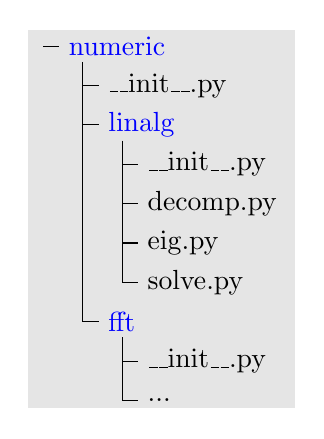
\begin{tikzpicture}
\fill[black!10!white] (-0.2,  0.2) rectangle (3.2, -4.6);
\draw (0.0,  0.0) -- (0.2,  0.0) node[anchor=west] {\color{blue}numeric};
\draw (0.5, -0.2) -- (0.5, -3.5);
\draw (0.5, -0.5) -- (0.7, -0.5) node[anchor=west] {\_\_init\_\_.py};
\draw (0.5, -1.0) -- (0.7, -1.0) node[anchor=west] {\color{blue}linalg};
\draw (1.0, -1.2) -- (1.0, -3.0);
\draw (1.0, -1.5) -- (1.2, -1.5) node[anchor=west] {\_\_init\_\_.py};
\draw (1.0, -2.0) -- (1.2, -2.0) node[anchor=west] {decomp.py};
\draw (1.0, -2.5) -- (1.2, -2.5) node[anchor=west] {eig.py};
\draw (1.0, -3.0) -- (1.2, -3.0) node[anchor=west] {solve.py};
\draw (0.5, -3.5) -- (0.7, -3.5) node[anchor=west] {\color{blue}fft};
\draw (1.0, -3.7) -- (1.0, -4.5);
\draw (1.0, -4.0) -- (1.2, -4.0) node[anchor=west] {\_\_init\_\_.py};
\draw (1.0, -4.5) -- (1.2, -4.5) node[anchor=west] {...};
\end{tikzpicture}
\end{column}
\begin{column}{7.3cm}
In jedem Paket-Ordner: \lstinline{__init__.py} \\
(kann leer sein)
\vspace{2mm}
\begin{lstlisting}[style=Python]
import numeric
numeric.foo() #Aus __init__.py
numeric.linalg.eig.foo()
\end{lstlisting}
\begin{lstlisting}[style=Python]
from numeric.linalg import eig
eig.foo()
\end{lstlisting}
\end{column}
\end{columns}
\end{frame}

%%% Local Variables: 
%%% mode: latex
%%% latex-run-command: pdflatex
%%% TeX-master: "vortrag"
%%% End: 

\section*{Ausnahmen}
\begin{aufgabe}
Lesen Sie vom Benuter eine Zahl ein und geben Sie ihr Quadrat aus. Was passiert, wenn der Benutzer etwas anderes als eine Zahl eingibt? Geben Sie eine benutzerfreundliche Fehlermeldung aus!
\end{aufgabe}

\begin{aufgabe}[Fakult"at erweitert]
Die Fakult"at ist nur f"ur nat"urliche Zahlen definiert. Wie reagiert die Funktion aus Aufgabe \ref{fakultaet} auf negative Parameter? Lassen Sie die Funktion in diesem Fall einen \texttt{ValueError} ausl"osen.
\end{aufgabe}

\begin{aufgabe}Schreiben Sie ein Programm, welches in einer Endlosschleife Eingaben vom Benutzer einliest und jeweils pr"uft, ob die Eingabe ein Palindrom ist (verwenden Sie die Funktion aus Aufgabe \ref{palindrom}). 

Was passiert, wenn der Benutzer \texttt{Ctrl-C} oder \texttt{Ctrl-D} dr"uckt? "Andern Sie das Programm, sodass der Benutzer beim Dr"ucken von \texttt{Ctrl-C} oder \texttt{Ctrl-D} gefragt wird, ob er das Programm beenden m"ochte.
\end{aufgabe}

\begin{aufgabe}
Mit dem Modul \texttt{readline} k"onnen f"ur die Benutzereingaben mittels \texttt{raw\_input} Editierm"oglichkeiten wie in der Shell aktiviert werden. Dieses Modul ist standardm"a"sig nur unter *nix-Systemen verf"ugbar. Folgender Code importiert das Modul nicht auf Windows-Rechnern:
\begin{lstlisting}
if not sys.platform.startswith("win"):
    import readline
    import rlcompleter
    readline.parse_and_bind("tab: complete")
\end{lstlisting}
Warum ist ein Ansatz mit Ausnahmen besser? Schreiben Sie den Code so um, dass er mit Ausnahmen arbeitet.
\end{aufgabe}

%%% Local Variables: 
%%% mode: latex
%%% TeX-master: "uebung1"
%%% End: 

\section*{Zus"atzliche Aufgaben}

\begin{aufgabe}[Zahlenraten]
Programmieren Sie das Spiel Zahlenraten: Ein Spieler (hier der Computer) denkt sich eine Zahl zwischen 1 und 100 aus, der andere Spieler (hier der Benutzer) muss die Zahl raten. Nach jedem Versuch erf"ahrt der Benutzer, ob er zu hoch, zu niedrig oder genau richtig lag. Eine Runde ist zuende, wenn die Zahl richtig geraden wurde.
\begin{teilaufgabe}
Das Programm l"asst den Benutzer eine Runde spielen und gibt am Ende die Anzahl der ben"otigten Versuche aus. \hinweis Eine Zufallszahl zwischen 1 und 100 wird mit dem Befehl \lstinline{random.randint(1, 100)} erzeugt.
\end{teilaufgabe}
\begin{teilaufgabe}
Das Programm fragt nach jeder Runde, ob der Benutzer noch einmal spielen m"ochte.
\end{teilaufgabe}
\begin{teilaufgabe}
Das Programm speichert eine Highscore-Liste in einer Datei.
\end{teilaufgabe}

\end{aufgabe}


%%% Local Variables: 
%%% mode: latex
%%% TeX-master: "uebung1"
%%% End: 


\vfill
\setlength{\fboxsep}{4mm}
\begin{center}
\fbox{\parbox{8cm}{\centering
War das nicht genug? Weitere Aufgaben:\\[2mm]
 \texttt{\underline{http://www.pythonchallenge.com}}
}}
\end{center}

\end{document}
